\begin{figure}[H]
    \centering
    \begin{tikzpicture}
        \pgfplotsset{
            width=1.0\textwidth,
            height=0.4\textheight
        }
        \begin{axis}
            [
                xbar=2pt,
                legend style={at={(0.5,-0.15)}, anchor=north,legend columns=-1},
                bar width = 5pt,
                xlabel= DEC (Joules),
                ylabel= Core,
                xmin=0,xmax=90,
                    ytick={0,1,2,3,4,5,6,7,8,9},
            ]
            \addplot coordinates { 
                (26.07,0)
                (26.29,1)
                (25.92,2)
                (25.92,3)
                (25.47,4)
                (26.29,5)
                (19.58,6)
                (19.39,7)
                (17.67,8)
                (19.47,9)
                };
            \addplot coordinates { 
                (26.61,0)
                (26.49,1)
                (26.32,2)
                (26.58,3)
                (25.93,4)
                (27.05,5)
                (33.87,6)
                (32.15,7)
                (31.03,8)
                (30.45,9)
                };
            \legend{NB, SN}
            \end{axis}
        \end{tikzpicture}
    \caption{DEC}
    % \caption{The average DEC for DUT 2, where both benchmarks are compiled on oneAPI}
\end{figure}
